\documentclass[12pt,a4paper,oneside,openright]{report}
%package for mathematics
\usepackage{amsmath,amssymb,amsfonts,mathptmx}
%package to include appendix
\usepackage[toc,page]{appendix}
%package for graphics
\usepackage{graphicx}
% package to insert 2 images side by side
\usepackage{float}
\usepackage{caption}
\usepackage{subcaption}
%package for inserting long tables on multiple pages
\usepackage{longtable}
\usepackage{array}
%package for list manipulation and tables
\usepackage{array,multicol,multirow,paralist}
%package for bullets
%\verb+ \usepackage{paralist} +
%package for typesetting margins
\usepackage[top=25.4mm, bottom=32mm, left=37mm, right=25.4mm]{geometry}
%\usepackage[margin=2cm]{geometry}
%package for hyperlinking
\usepackage[colorlinks=true,linkcolor=black,citecolor=blue]{hyperref}
%package to set line spacing
\usepackage{setspace}
%usepackage for page style
\usepackage[Lenny]{fncychap}
\usepackage{wallpaper}
\usepackage{fancyhdr}
\pagestyle{fancy}
%\titleformat{\section}{\large\bfseries}{\thesection}{1mm}
\usepackage{times}
%\lhead{\scriptsize \textsc{ME (EnTC)}} %left header
%\chead{\footnotesize \leftmark} %center header %leftmark is chapter name
\chead{}
\rhead{}
\lhead{\scriptsize \textsc{Smart Ambulance With Traffic Clearance}}
%\rhead{\footnotesize \rightmark} %right header %rightmark is the first section that appears on that page
\cfoot{\footnotesize \textsc{SITS, Narhe, Pune-41 (E \& TC Engineering)\\ \thepage}} %left footer
%\cfoot{\footnotesize ME (E\& TC)} %right footer
%\rfoot{\footnotesize \thepage} %center footer
\renewcommand{\headrulewidth}{0.5mm}	%we cant pass the values to headrulewidth directly so we have to use renewcommand
\renewcommand{\footrulewidth}{0.5mm}
%\newfont{\selectfont}{Times new roman}
\setcounter{secnumdepth}{4}
\setcounter{tocdepth}{3}
\renewcommand{\headrulewidth}{0.5pt}
\renewcommand{\footrulewidth}{0.5pt}
\newcommand{\HRule}{\rule{\linewidth}{0.5mm}}

\usepackage{tabulary}
\newcolumntype{K}[1]{>{\centering\arraybackslash}p{#1}}
\usepackage{gensymb}
\usepackage[utf8x]{inputenc}
\usepackage{listings}
\usepackage{titlesec}
\usepackage{lipsum}

\titleformat{\chap}[display]
{\normalfont\Large\filcenter\sffamily}
{\vspace*{\fill}
 \titlerule[1pt]%
 \vspace{1pt}%
 \titlerule
 \vspace{1pc}%
 \LARGE\MakeUppercase{\chaptertitlename}~\thechapter}
{1pc}
{\titlerule\Huge}
[\vspace*{\fill}\newpage]












\begin{document}


% Title page

\begin{titlepage}
% \ThisCenterWallPaper{1}{../img/pb1}
\begin{center} \vspace*{6mm}
\textbf{\textsc{a}} \\[2mm]
\textbf{\textsc{Project Report}}\\[2mm]
\textbf{\textsc{on}}\\[6mm]
\textbf{\textsc{\Large{Smart Ambulance With Traffic Clearance}}}\\[8mm]
\textbf{\textsc{\normalsize{submitted to the savitribai phule pune university,\\ in the partial fulfillment of requirements
for the award of the degree
}}}\\[4mm]
\textbf{of} \\[6mm]
\textbf{\textsc{\Large{BACHELOR OF ENGINEERING \\ \vspace{.5cm}  (ELECTRONICS AND TELECOMMUNICATION)}}}\\[8mm]
\textbf{by}\\[4mm]

\begin{tabular}{l l l }
\textsc{\bf Ranveer Kumar}  & Exam seat No. &: \texttt{\bf B120573116}\\
\textsc{\bf Rajesh Kumar} &Exam seat No. &: \texttt{\bf B120573114}\\
\textsc{\bf Shreyesh Ragit} &Exam seat No. &: \texttt{\bf B120573134}\\
\end{tabular}
\\[5mm]
\textit{UNDER THE GUIDANCE OF}\\[4mm]
\textsc{\bf Mr. N. S. Kulkarni}\\[8mm]


\includegraphics[scale=0.7]{Figures/logo.png}\\[8mm]
\textbf{\textsc{\large{DEPARTMENT}} OF \textsc{\large{E\&TC ENGINEERING}}}\\[6mm]
\textbf{\textsc{\footnotesize{SINHGAD TECHNICAL EDUCATION SOCIETY'S}}}\\[3mm]
\textbf{\textsc{\large{SINHGAD INSTITUTE}} OF\textsc{\large{ TECHNOLOGY \& SCIENCE}}}\\[3mm]
\textbf{\textsc{\small{NARHE (AMBEGAON), OFF WESTERLY BY PASS PUNE MUMBAI EXPRESSWAY, }}}\\[3mm]
\textbf{\textsc{\footnotesize{NARHE,PUNE - 411 041}}}
\end{center}
\end{titlepage}

% Certificate page 

\begin{titlepage}
% \ThisCenterWallPaper{1}{../img/pb1}
\begin{center} \vspace*{20mm}
\thispagestyle{empty}
\onehalfspacing
{\large \textsc{CERTIFICATE}} \\[5mm]
\textsc{this is to certify that the project report entitled}\\[3mm]
\textbf{"Smart Ambulance With Traffic Clearance"}\\[3mm]
\textsc{submitted by}\\[3mm]
\begin{tabular}{l l l }
\textsc{\bf Ranveer Kumar}  & Exam seat No. &: \texttt{\bf B120573116}\\
\textsc{\bf Rajesh Kumar} &Exam seat No. &: \texttt{\bf B120573114}\\
\textsc{\bf Shreyesh Ragit} &Exam seat No. &: \texttt{\bf B120573134}\\
\end{tabular}
\\[7mm]
\end{center}
\textsc{is a bonafide work carried out by them under the guidance of \textbf{Mr. N.S.Kulkarni } and it is approved for the partial fulfillment of the requirement of the savitribai phule pune university for the award of 
\begin{center}
Bachelor degree of engineering in\\ \textbf{(E\&TC Engineering)} 
\end{center}
this project report has not been earlier submitted to any other institute of university for the award of any degree or diploma.\\[10mm]}

\begin{center}
\begin{tabular}{K{5cm}K{5cm}K{5cm}}
\textbf{Mr. N. S. Kulkarni}	& 	\textbf{Mr. S.B. Shrote}		&\textbf{Mr.  D. E. Upasani}\\
Project Guide		&	Project Co-Ordinator	&Head Dept. of E\&TC\\
Dept. of E\&TC		&	Dept. of E\&TC		&SITS, Pune, 411041\\
SITS, Pune, 411041	&	SITS, Pune, 411041	&\\[3cm]

			&\bf Dr. S. N. Mali&\\
&Principal&\\
&SITS, Pune, 411041&\\
\end{tabular}
\end{center}
\vspace{1cm}
\begin{flushleft}
\textbf{Place}: Pune\\
\textbf{Date} : 
\end{flushleft}
\end{titlepage}

\newpage
\pagenumbering{gobble} %gobble creates new page numbering style
\pagenumbering{roman} %roman creates roman numbers
% tABLE OF CONTENT

\tableofcontents

\begin{center}
\chapter*{Acknowlegement}	%when we use star we dont get any number in the contents but still it appears in the contenrs 
\end{center}
\addcontentsline{toc}{chapter}{Acknowledgement}
\doublespacing

I express my profound gratitude towards respected guide \textbf{Mr. N. S. Kulkarni} and, Project Coordinator \textbf{Mr. S. B. Shrote} for their constant encouragement and valuable guidance during completion of my present work. They are the true guide who guided me with moral values.
	I am also thankful to H.O.D (E\&TC dept.) \textbf{Mr. D. E. Upasani} for supporting me in conception of project works as well as providing guidelines time to time.
	I am deeply indebted and I would like to express my sincere thanks to the Principal \textbf{Dr. S. N. Mali} sir for his support.
I take this opportunity to thank all staff members of E \& TC Dept. for their co-operation and help during this work.
Finally, I express my honest and sincere feelings towards all those who directly or indirectly encouraged me, helped me, and criticized me in accomplishment of my present work.

\vspace{2cm}

\begin{flushright}
\textbf{Ranveer Kumar}(B120573116)\\
\textbf{Rajesh Kumar}   (B120573114)\\
\textbf{Shreyesh Ragit} (B120573134)
\end{flushright}
\hfill
\pagebreak

\addcontentsline{toc}{chapter}{List of Figures}
\listoffigures
\newpage
\addcontentsline{toc}{chapter}{List of Tables}
\listoftables
\newpage
\addcontentsline{toc}{chapter}{Abstract}
\chapter*{Abstract}
\doublespacing
Normally, in an ambulance facilities such as blood pressure measurement, or glucose to the patient, or first aid are provided in an ambulance. Here we are looking at what additional treatments can be provided and how to send all the medical details to the hospital where the patient is being taken so that all the preparations required can be done before the patient reaches the hospital. After discovering and going through all these points, we are coming up with an idea to implement a system, where we get the medical record of the patient, e.g , blood group, any previous medical issues, and sending them to the hospital . Along with this, we are also providing this idea where we are using a traffic clearance system with the help of IR sensors. Ambulances have the IR transmitter which transmits the Infrared signal (IR). IR-LED (Light Emitting Diode) is connected in series for better range and wider directivity. This module can transmit IR rays up to few meters without use of any external lens. IR receivers are placed just a few meters before the traffic signals to clear the signal when they sense any emergency medical van coming in its directions by turning the signal green for that path. The receiver uses infrared module (photodiode). The output of the photodiode is connected to microcontroller. Along with this concept, the concept of GSM (Global System for Mobile Communication) is also being used, by which Doctor of particular specialization, as needed by the patient, is messaged to report to the Hospital before the arrival of ambulance.


\newpage
\pagenumbering{gobble}
\pagenumbering{arabic}	%all the chapters will have arabic numbers



\newpage
\vspace*{\fill}
 \begin{center}
\hrule%
\vspace{1pt}%
\hrule
\vspace{1pc}%
\LARGE\MakeUppercase{INTRODUCTION} 
\vspace{1pc}%
\hrule%
\vspace{1pt}%
\hrule
 \end{center}
 \vspace*{\fill}

% \chap{INTRODUCTION}
\chapter{INTRODUCTION}
\section{Background}
In today’s world health hazards are a major concern. Especially people in the older age group are the victims, and moreover the traffic conditions are worsening day by day, which results in traffic jams. Many emergency cases get delayed due to these traffic jams.   Ambulance service is one of the major services which gets affected by traffic jams. To solve this problem we have come up with the solution of \textbf{“Smart ambulance with automatic traffic clearance”}.

The primary role of all ambulance service is emergency pre – hospital medical care, although they generally provide both emergency response and patient transfer on behalf of the health sector. They provide easy access to health services, particularly out of hours , and contribute significantly to telephone triage and telephone health services through sophisticated communications infrastructure . In recent times it has become apparent that increasing health system pressures cannot be resolved only by adding resources, but must also be addressed with new methods of service delivery. If ambulance services can develop towards an out-of-hospital, clinical care service rather than merely pre-hospital clinical care, they could substantially add to functionality of the health system. This could be through more efficient transfer of patient information; more efficient movement of patients an ambulance service with a public service rather than profit driven philosophy; and patient treatment regimens consistent with the broader health system.

\subsection{Ambulance Unit}
With reference to paper [2], we are tracking the patient’s health conditions. The health parameters such as Heart rate, body temperature, Blood pressure and Blood level are sent to the hospital using the on board GSM unit. All these parameters are displayed in the hospital unit on a pc with the help of s/w.

\subsection{Traffic Unit}
Simultaneously if at all the Ambulance encounters the traffic jam in the route, the ambulance can be given the priority by controlling the traffic signals using IR sensors. The particular signal is made Green for some time and after the ambulance passes by, it again regains its original flow of sequence of signalling.
\begin{figure}[!h]
 \centering
 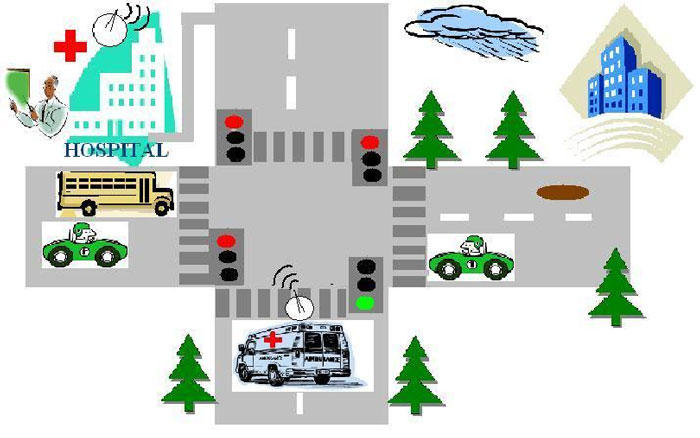
\includegraphics[width = \textwidth]{Figures/fig_1.png}
 \caption{Logical block diagram of the system proposed}
 \label{bdm}
\end{figure}

As we can observe there is a chowk shown in the Figure:\ref{bdm} , consisting of four different lanes. An ambulance is going from lane1. The patient is carried in the medical van, whose various parameters are being measured by the sensory units inside the van. These parameters are constantly being sent to the hospital unit via GSM transreceiver, [3] “A Hardware based approach in designing Infrared Traffic Light System” , in the form of a message of data (SMS). The hospital you can see is at the side of road and it is receiving these SMS’s via a dedicated mobile phone. The information is shown on the pc connected to this mobile phone via data cable.

At the same time, when the ambulance is reaching the signal of lane 1, the signal turns green and all other signals as red. This will be achieved by IR sensors, used in the ambulance and across the road near the signal. 

\section{Relevance}
In today’s world health hazards are a major concern. Especially people in the older age group are the victims, and moreover the traffic conditions are worsening day by day, which results in traffic jams. Many important jobs get delayed due to these traffic jams. Ambulance service is one of the major services which gets affected by traffic jams. To solve this problem we have come up with the solution of “Intelligent ambulance with automatic traffic control”. Here we are tracking the patient’s health conditions. The health parameters such as Heart rate, body temperature, Blood pressure and Blood level are sent to the hospital using the on board GSM unit. All these parameters are displayed in the hospital unit on a pc with the help of visual basic s/w. Simultaneously if at all the Ambulance encounters the traffic jam in the route, the driver is provided with the remote to control the traffic signals. The particular signal is made Green for some time and after the ambulance passes by, it again regains its original flow of sequence of signalling.

\newpage
\vspace*{\fill}
 \begin{center}
\hrule%
\vspace{1pt}%
\hrule
\vspace{1pc}%
\LARGE\MakeUppercase{LITERATURE SURVEY} 
\vspace{1pc}%
\hrule%
\vspace{1pt}%
\hrule
 \end{center}
 \vspace*{\fill}

\chapter{LITERATURE SURVEY}
\section{Introduction}
In the introduction we have explained the general information of an ambulance and traffic clearance. The aim of the project is to propose a solution of “Intelligent ambulance with automatic traffic control”. We first started by researching on the basics of ambulance services and about its processing. We then explored what else can be provided to a patient on its way to hospital can be . We also looked at how to send these medical details back to the hospital where the patient is being taken to.

Previous work on home vital signs monitoring can be seen in the current models that are available in home and hospitals. There are many various types and brands of vitals available today.  They vary in range, size , and functions . Most are very expensive costing patients or health care providers of \$ 2500 per system. There are many different types of vital signs monitors , so many patients vital signs monitor exist. One such patient is a blood pressure and heart monitoring method and apparatus by Hewitt. This system uses an ausculatory transducer and a microprocessor based circuit to record blood pressure and heart rate. It also uses a new method to measure blood pressure without necessary constriction of the patient’s limbs. So far in the market only the devices measuring different parameters are available which are all stationary, but we are putting efforts to send this information wirelessly over the long distance using gsm unit.

It is the process of providing acute medical treatment provided to the patient on the way up to hospital which involves a series of communication between devices of the hospital and ambulance unit. The project is based on providing a smart ambulance with traffic light control system,  i.e. providing a better medical attention to the patient on its way up  to the hospital and also controlling the traffic light in case a heavy traffic is met on a signal while taking the patient to the hospital, that drives to reset the traffic light to green light at ambulance side and red light at other three sides. 

Ayush Kr. Mittal and Deepika Bhandari proposed a green wave system. It is used to provide clearance to any emergency vehicle by turning all the red lights to green on the path of the emergency vehicle, for this reason providing a complete green wave to the desired vehicle. A “green wave” is the synchronization of the green phase of traffic signals. With a “green wave” setup , a vehicle passing through a green signal will continue to receive green signals as it travels down the road. Advantage of the system is that GPS inside the vehicle does not require additional power. The biggest disadvantage of green waves is that, when the wave is disturbed then the disturbance can cause traffic problems. 

Gargi Beri, Pankaj Ganjare, Amruta Gate, and Ashwin Channawar’ in \textbf{“Intelligent Ambulance with Traffic Control”} , says , ambulance service is one of the crucial services that get delayed very often. Also sometimes on sight doctors are not available. So the patient does not get medical attention immediately. To overcome such situation, this paper describes a solution that is ‘Intelligent ambulance with traffic control’ which includes intelligent traffic controlling as well as a health monitoring system. Here the goal is to reduce the latency of emergency vehicles with minimum or less disruption to regular traffic flow is possible. Ambulances have a transmitter which transmits the Infrared signal (IR). IR-LED (Light Emitting Diode) is connected in series for better range and wider directivity. This module can transmit IR rays up to few meters without use of any external lens. Traffic light has a receiver. The receiver uses infrared module (photodiode). The output of the photodiode is connected to microcontroller.. Along with this concept, [5] “A Review Paper on Design of GPS and GSM Based Intelligent Ambulance Monitoring” the concept of GPS and  GSM (Global System for Mobile Communication) is also being used, by which Doctor of particular specialization, as needed by the patient, is messaged to report to the Hospital before the arrival of ambulance. SIM 900 is used for Serial communication and the message is displayed in a 16x2 LCD (Liquid Crystal Display) connected to the receiver. GSM here, not only used for just sending message to the doctor but also used for video display of the patient in the ambulance using 3G connection. By which Doctor can analyse the condition of the patient and recommend some immediate possible medical attention in ambulance before reaching hospital.

The research paper on \textbf{“An Advance Intelligent Ambulance With Online Patient Monitoring System”}, says , the traffic congestion problems are the phenomenon which contributed huge impact to the transportation system. Ambulance service is one of the major services which get affected by traffic jams. So many important schedules get delayed due to these traffic jams. To solve this problem we have come up with the solution of “An Advance Intelligent Ambulance With Online Patient Monitoring System”. In this, we will track the patient’s health conditions with following parameters such as heart rate, body temperature, etc. These parameters are sent to any specified cell phone using GSM unit. This system is designed to operate the traffic light, when it receives signals from an emergency vehicles whose signal transmissions are based on radio frequency (RF). This system used 8052, AVR micro-controller for triggering purposes to change the normal state to the emergency state. Here we use an assembly programming for better accuracy and GPS and GSM modules which will trace the vehicle anywhere on the globe. According to this project, when patient’s parameters exceed the normal values then the sensor will detect the signal and sends it to micro-controller. The micro-controller will send the alert message through the GSM to an authorized mobile number, which will help in providing better facilities to the patient.

Research paper on \textbf{“A Hardware based approach in designing Infrared Traffic Light System”} says, nowadays, a traffic light is currently used to control the traffic at the road. The trend is clear that the technology of the traffic light is growing rapidly. However, there is still problem for the emergency vehicles to bypass when the traffic light is red. This is because the emergency vehicle is unable to reach the destination in short as well as there is an emergency case. So, the purpose of this project is to solve this problem. This paper presents the design of traffic light system that response for emergency vehicles to immediately bypass the traffic light. Hence, the emergency vehicle can reach the destination at the right time to save lives. 

The research paper \textbf{“A  Review Paper on Design of GPS and GSM  Based  Intelligent Ambulance”}, Monitoring  International  Journal  of  Engineering Research  and  Applications  , helps with the idea of using gps and gsm in the ambulance unit , to find out the location of the ambulance using gps and transmitting the data to the hospital unit through gsm. 

Proposed paper presents design of such a monitoring system for emergency patient transportation employing use of microcontroller module. The system will be useful for monitoring ambulance location using Googles map. It also include biomedical sensors to monitor heart bit rate and temperature of patient through SMS. The front end application at the monitoring system is developed using visual basic software in Personal Computers. It can display location of ambulance and status of heart bit rate and temperature of patient. After receiving SMS hospital can prepare their staff for proper treatment of coming patient.


\newpage
\vspace*{\fill}
 \begin{center}
\hrule%
\vspace{1pt}%
\hrule
\vspace{1pc}%
\LARGE\MakeUppercase{SYSTEM  DESIGN} 
\vspace{1pc}%
\hrule%
\vspace{1pt}%
\hrule
 \end{center}
 \vspace*{\fill}

\chapter{SYSTEM  DESIGN}
The system is designed to clear the heavy traffic, using RF transmitter and receiver, that is encountered more often than not in big cities especially at the traffic signals. The ambulance unit has sensors like, heartbeat sensor and temperature sensor to measure he body parameters of the patient. It also has gps and gms to find the location of the ambulance and to send the recorded body parameters of the patient to the hospital.

\section{Block Diagram}

\begin{figure}[!h]
 \centering
 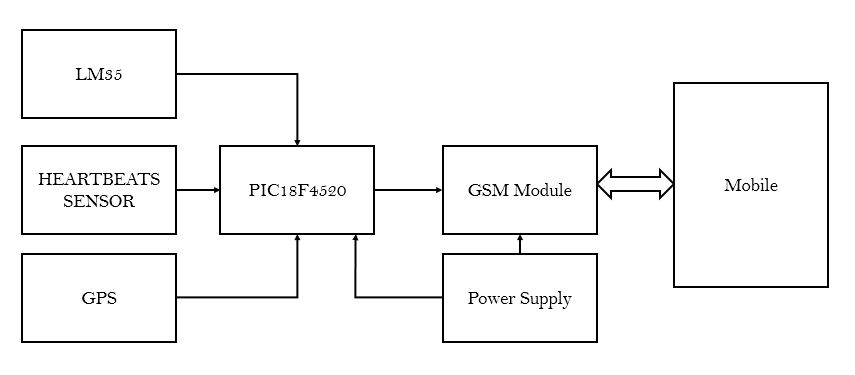
\includegraphics[width = .89\textwidth]{Figures/fig_2.png}
 \caption{Block diagram of Smart Ambulance}
 \label{bd}
\end{figure}

Figure:\ref{bd} shows the Block Diagram of Smart Ambulance System, containing all modules naming,
\begin{itemize}
 \item Sensors unit
 \item Controller unit
 \item Transmitter unit
 \item Supply unit
\end{itemize}

\begin{figure}[!h]
 \centering
 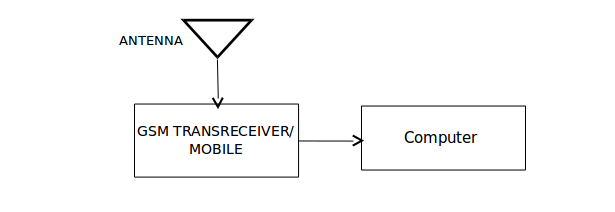
\includegraphics[width = .70\textwidth]{Figures/fig_3.png}
 \caption{Hospital Unit Block Diagram}
 \label{hbd}
\end{figure}
Figure:\ref{hbd} shows the Hospital Unit, Transmitted data received though GSM and send to Computer.

% \subsection{Ambulance Unit}
% \subsection{Hospital Unit}
\section{System Description}
\subsection{PIC 18F4520}
The advantages of all PIC18F4520 microcontroller– namely, high computational performance at an economical price – with the addition of high endurance, 
\begin{figure}[h]
 \centering
 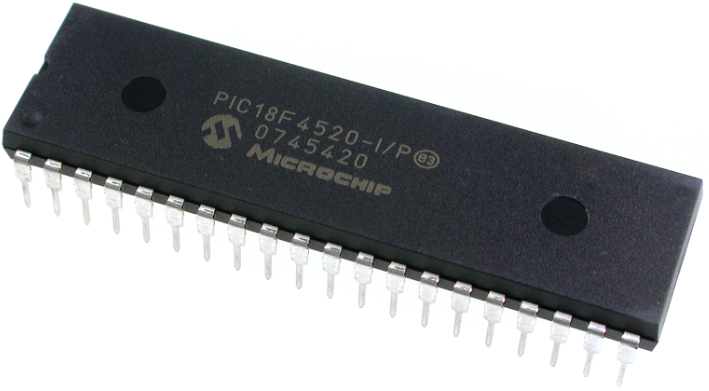
\includegraphics[width = .31\textwidth]{Figures/fig_4.png}
 \caption{PIC 18F4520}
 \label{uc}
\end{figure}
Enhanced Flash program memory ,introduces design enhancements that make these microcontrollers a logical choice for many high performance, power sensitive applications.

\subsubsection{Features}
\begin{itemize}
 \item \textbf{CPU}
 \begin{enumerate}
  \item Up to 10 MIPS Performance at 3V
  \item C compiler optimized RISC architecture
  \item 8x8 Single Cycle Hardware Multiply
 \end{enumerate}
\item \textbf{System}
\begin{enumerate}
  \item Internal oscillator support-31 kHz to 8MHz with 4xPLL
  \item Watchdog Timer with separate RC oscillator
  \item Wide operating Voltage range; 2.0V to 5.5V
\end{enumerate}
\item \textbf{NanoWatt Power Managed Modes} 
\begin{enumerate}
 \item Run, Idle and SLEEP modes
  \item Idle mode currents down to 5.8uA typical
  \item Sleep mode currents down to 0.1uA typical
\end{enumerate}
\item \textbf{Analog Features} 
\begin{enumerate}
 \item 10-bit ADC, 13 channels, 100K samples per second
  \item Programmable Low Voltage Detection Module
  \item Programmable Brown-out-Reset Module
\end{enumerate}
\item \textbf{Peripherals}
\begin{enumerate}
 \item Master Synchronous Serial Port
  \item Four Timer modules
  \item Four Crystal modes, up to 40 MHz
  \item 4X Phase Lock Loop (available for crystal and internal oscillators)
%   \item Two External RC modes, up to 4 MHz 
\end{enumerate}

\begin{figure}[!h]
 \centering
 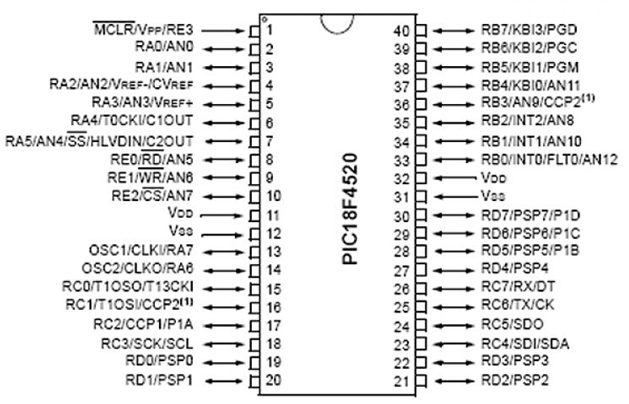
\includegraphics[width = .69\textwidth]{Figures/fig_5.png}
 \caption{Pin diagram of PIC18F4520}
 \label{pindiag}
\end{figure}

\item \textbf{Architecture of PIC18F4520}
\begin{figure}[!h]
 \centering
 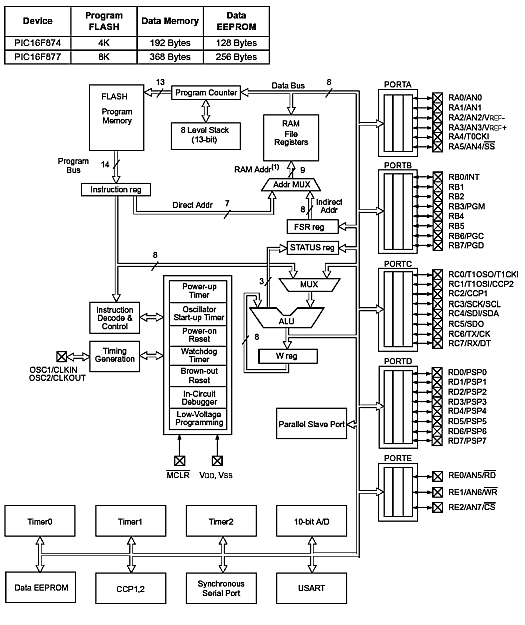
\includegraphics[width = .80\textwidth]{Figures/fig_6.png}
 \caption{Architecture of PIC18F452}
 \label{archuc}
\end{figure}
\end{itemize}

\subsection{Liquid Crystal Display}
LCD is used in a project to visualize the output of the application. We have used 16x2 LCD which indicates 16 columns and 2 rows. So, we can write 16 characters in each line. So, total 32 characters we can display on 16x2 LCD. LCD can also be used in a project to check the output of different modules interfaced with the microcontroller. Thus LCD plays a vital role in a project to see the output and to debug the system module wise in case of system failure in order to rectify the problem.

\subsubsection{LCD Power Sources}
\begin{enumerate}
 \item LCD has 2 Power Sources1. VCC and GND are at 1 and 2 NO. Pins of LCD. Used to drive the LCD 3 mA current consumption.
\item VCC and GND is at 15 and 16 NO. pins of LCD used to drive the backlight of LCD  100 mA current,
\end{enumerate}
\begin{align}
Total\, current\, consumption = 3mA + 100mA = 103 mA 
\end{align}
So, in order to reduce the current requirement we are connecting a 330 ohm resistance in series with the backlight pin VCC. This reduces the current consumption (100mA / 330ohm =0.303 mA).
Therefore,
\begin{align}
New total current consumption = 0.303mA+3 mA =3.303 mA 
\end{align}
\subsubsection{LCD Data and Control lines}
LCD has 8  / 4 data lines and 3 control lines .The 4 data lines of LCD (pin 11 to pin 14 ) are connected to the B port of PIC µC (B4 to B7) . The control lines of LCD are RS,R/W ,E. 
\subsubsection{Register Select (RS)}
The LCD RS pin is for selecting the data or the code register, it connected to pin 35 i.e. B2. If RS=0 , the instruction command code register is selected, allowing the user to send a command such as clear display , cursor at home, etc. If RS=1, the data register is selected, allowing the user to send data to be displayed on the LCD.
Read/ Write (R/W)
\begin{enumerate}
 \item The LCD R/W is for choosing between reading or writing on LCD. 
\item R/W=1 when reading, R/W=0 when writing.
\item Here R/W is connected to ground ie R/W=0.
\end{enumerate}

\subsubsection{Enable (E)}
\begin{enumerate}
 \item LCD pin E is for enabling or disabling the LCD which connected to pin 34 i.e. B1.
\item The enable pin is used by the LCD to latch information presented to its data pins. a high-to- low pulse must be applied to this pin.
\end{enumerate}

\begin{figure}[!h]
 \centering
 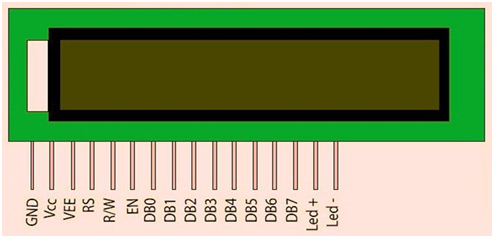
\includegraphics[width = .90\textwidth]{Figures/7.jpg}
 \caption{16 * 2 LCD}
 \label{lcd}
\end{figure}
LCD can also be used in a project to check the output of different modules interfaced with the microcontroller. Thus LCD plays a vital role in a project to see the output and to debug the system module. 

This Table shows Pin Description of LCD Pin as below:

\begin{table}[!h]
\centering
\caption{Pin Description of LCD}
 \begin{tabular}{|l|l|l|} \hline
 \bf Pin No.	&\bf Symbol & \bf Function \\ \hline
1		&GND	&GROUND		\\	\hline
2		&VCC	&+ 5 V	\\ \hline
3		&CONTRAST &GND \\ \hline
4		&E	&ENABLE \\ \hline
5		&RS	&REGISTER SELECT \\ \hline
6		&R/W	&READ WRITE \\ \hline
7		&DB0	&DATA LINE \\ \hline
8		&DB1	&DATA LINE \\ \hline
9		&DB2	&DATA LINE \\ \hline
10		&DB3	&DATA LINE \\ \hline
11		&DB4	&DATA LINE \\ \hline
12		&DB5	&DATA LINE \\ \hline
13		&DB6	&DATA LINE \\ \hline
14		&DB7	&DATA LINE \\ \hline
15		&VCC	&+ 5 V \\ \hline
16		&GND	&GND \\ \hline
 \end{tabular}
\end{table}

\subsection{Temerature Sensor}
Temperature sensor is used to sense the temperature. We have used a Temperature sensor called LM35. This temperature sensor can sense the temperature of the atmosphere around it or the temperature of any machine to which it is connected or even can give the temperature of the human body in case if used. So, irrespective of the application to which it is used, it gives the reading of the temperature. 
\begin{figure}[!h]
 \centering
 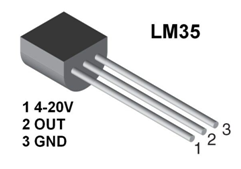
\includegraphics[width = .30\textwidth]{Figures/8.jpg}
 \caption{Temperature sensor LM35}
 \label{lm35}
\end{figure}
The LM35 series are precision integrated-circuit temperature sensors, whose output voltage is linearly proportional to the Celsius (Centigrade) temperature.
\subsubsection{Features}
\begin{enumerate}
 \item Calibrated Directly in Celsius (Centigrade)
\item Linear +10-mV/C Scale Factor 
\item 0.5°C Ensured Accuracy (at 25°C)
\item Rated for Full −55°C to 150°C Range
\item Suitable for Remote Applications
\item Low-Cost Due to Wafer-Level Trimming
\item Operates from 4 V to 30 V
\item Less than 60-$\mu$A Current Drain
\item Low Self-Heating, 0.08°C in Still Air
\item Non-Linearity Only ±¼°C Typical
\item Low-Impedance Output, 0.1$\Omega$ for 1-mA Load
\end{enumerate}

\subsubsection{Applications}
\begin{enumerate}
 \item Power Supplies
\item Battery Management
\item HVAC
\item Appliances
\end{enumerate}

\subsection{Heartbeat Sensor}
It is designed to provide analog output of heart beat when a finger is placed on it. When the Heart detector starts working, the top most LED will starts flashing with every heart beat. The output of this sensor can be connected to Micro Controller directly to measure the heart beat. It functions on the principle of light modulation by blood flow through the nerves of the finger at every pulse. The module output mode, analog output mode is simple. 

\begin{figure}[!h]
 \centering
 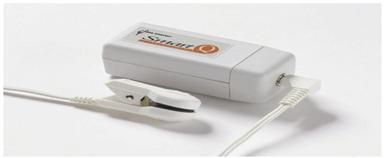
\includegraphics[width = .80\textwidth]{Figures/9.jpg}
 \caption{TCRT1000}
 \label{TCRT1000}
\end{figure}
It is having 4 pins.  Pin1: To give supply voltage to the LED. Pin2 and 3 are grounded. Pin 4 is the output. Pin 1 is also the enable pin and pulling it high turns the LED on and the sensor starts working. It is embedded on a wearable device which can be worn on the wrist and the output can be sent wirelessly (through Bluetooth) to the computer for processing. The TCRT1000 is reflective sensors which include an infrared emitter and phototransistor in a leaded package which blocks visible light.

\subsubsection{Features}
\begin{enumerate}
 \item Package type: leaded
\item Detector type: phototransistor 
\item Dimensions (L x W x H in mm): 7 x 4 x 2.5 
\item Peak operating distance: 1 mm 
\item Operating range within $>$ 20 % relative collector current: 0.2 mm to 4 mm 
\item Typical output current under test: IC = 0.5 mA 
\item Daylight blocking filter 
\item Emitter wavelength: 950 nm 
\item Lead (Pb)-free soldering released
\end{enumerate}
\subsubsection{Applications}
\begin{enumerate}
 \item Optoelectronic scanning and switching devices i.e., index sensing, coded disk scanning etc. (optoelectronic encoder assemblies for transmission sensing).
\end{enumerate}


\subsection{ECG}
ECG is an electrocardiogram system in which electrical activity of the heart is recorded via electrodes placed on body. Here 2-lead Ag-Cl electrodes along with conducting gel (to reduce the skin resistance) are used. ECG signal is of a very small amplitude (1mV- 5mV).Electrodes measure the impulse signals (Bio-potential signals) generated by the heart which are transferred to the surface of the body.
\begin{figure}[!h]
 \centering
 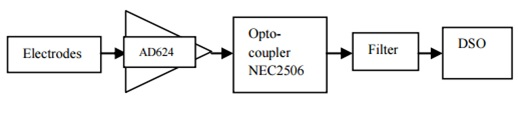
\includegraphics[width = \textwidth]{Figures/10.jpg}
 \caption{Block diagram of ECG}
 \label{becg}
\end{figure}
Figure:\ref{becg} shown is the block diagram of an electrocardiogram containing:
\begin{itemize}
 \item Electrodes
 \item AD624
 \item Opto-cupler
 \item Filter
 \item DSO
\end{itemize}

AD624AD is an analog instrumentation amplifier IC used to amplify signals generated due to contraction and relaxation of heart. The AD624 is set up with a gain of 1000, and is supplied by +9 V and -9V power supply. Opto-coupler NEC2506 is used to isolate the input of amplifier from the rest of the circuitry. Band pass filter containing low-pass and high-pass filters are used with the RC \& time constants. 

\begin{figure}[!h]
 \centering
 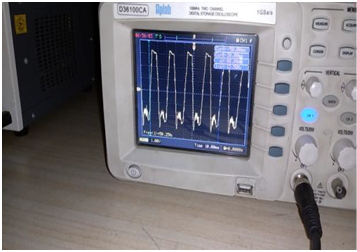
\includegraphics[width = .80\textwidth]{Figures/11.jpg}
 \caption{ECG measurement(Electrocardiogram)}
 \label{mecg}
\end{figure}

\subsection{HT12E and TX4333}
Ht12e Is Basically an Rf Encoder. It Gets The Coded 4bit Data From Pic At Its Data  Pins. The Ht12e Then Generates A Digital Pulse Signal With 1 Redundant 8 Address And 4 Data Bits Encoded By Pic. The Encoded 4 Bit Data Is Different Fir The Four Lanes. This 13 Digital Bit String Is Again Modulated Using Fsk And Send At A Frequency Of 433mhz , This Is Done By Tx433 And Rf Tx. It’s Range Is About 100 Meter .
% lambda problem
\subsection{GSM}
The concept of GSM (Global System for Mobile Communication) is also being used, by which Doctor of particular specialization, as needed by the patient, is messaged to report to the Hospital before the arrival of ambulance. SIM800C is a quad-band GSM/GPRS module that works on frequencies GSM850MHz, EGSM900MHz, DCS1800MHz and PCS1900MHz. SIM800C features GPRS multi-slot class10/class12 (optional) and supports the GPRS coding schemes CS-1, CS-2, CS-3 and CS-4. With a tiny configuration of 17.6*15.7*2.3mm, SIM800C can meet almost all the space requirements in customers’ applications, such as smart phone, PDA and other mobile devices. SIM800C is a SMT package with 42 pads, and provides all hardware interfaces between the module and customers’ boards.  One 3 lines serial port and one full modem serial port;$\lambda$  One USB, the USB interface can debug, download software;  One audio channel which include a microphone input and a speaker output;  Programmable general purpose input and output;$\lambda$  One SIM card interface; $\lambda$  Support Bluetooth (need software support). $\lambda$ SIM800C is designed with power saving technique so that the current consumption is as low as 0.6mA in sleep mode.

\begin{table}[!h]
\centering
\caption{SIM800C Module information}
 \begin{tabular}{|l|l|}\hline
 \bf MICROCONTROLLER & \bf PIC18F4520 \\ \hline
GSM  	&850,900,1800 and 1900MHz \\ \hline
BT	&(need software support) \\ \hline
FLASH & SIM800C (24Mbit) \\
      &SIM800C32 (32Mbit) \\ \hline
RAM	&32Mbit \\ \hline
 \end{tabular}
\end{table}
\subsection{GPS}
Global Positioning System (GPS) satellites broadcast signals from space that GPS receivers, use to provide three-dimensional location(latitude, longitude,and altitude) plus  precise time. GPS receivers provides reliable positioning, navigation, and timing services to worldwide users on a continuous basis in all weather, day and night, anywhere on or near the Earth. The output is serial data of 9600 baud rate which is standard NMEA 0183 v3.0 protocol offering industry standard data messages and a command set for easy interface to mapping software and embedded devices. The current GPS consists of three major segments. These are the space segment (SS), a control segment (CS), and a user segment (US)

This GPS Receiver Modem is based on SIMCOM' Sim28M/Sim28 ML GPS Module. SIM 28 ML is stand-alone or A-GPS receiver with build in LNA. SIM 28M can relex antenna requirement and don’t need for external LNA. Sim 28ML can track as low as -165 dbi signal even without etwork assistance.SIM 28ML has excellent low power consumption characteristics(acquisition 17mA, tracking 16 mA). Sim 28ML supports various location and navigation applications including autonoums GPS, QZSS,SBAS ranging (WASS, EGNOS, GAGAN, MSAS). DGPS and A-GPS.

\begin{figure}[!h]
 \centering
 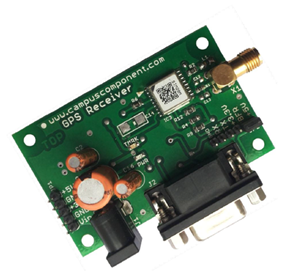
\includegraphics[width = .50\textwidth]{Figures/12.jpg}
 \caption{GPS module}
 \label{gps}
\end{figure}

\subsubsection{Features}
\begin{enumerate}
 \item Serial interfaces: UART, SPI / I2C
\item Digital I/O: EINT0 input, GPIO ,Time pulse
\item Protocols: NMEA ,PMTK
\item Electrical Data:
  \begin{enumerate}
   \item Power supply 2.9V to 3.6V
  \item Backup power 3.0V
\item Power consumption
\item Antenna type Active and passive
  \end{enumerate}
\end{enumerate}


\subsection{IR Sensor}
The system contains IR transmitter and IR receiver which are mounted on the either sides of roads respectively. The IR system gets activated whenever any vehicle passes on road between IR transmitter and IR receiver. Microcontroller controls the IR system and counts number of vehicles passing on road. Microcontroller also store vehicles count in its memory. Based on different vehicles count, the microcontroller takes decision and updates the traffic light delays as a result. The traffic light is situated at a certain distance from the IR system. Thus based on vehicle count, microcontroller defines different ranges for traffic light delays and updates those accordingly.

\begin{figure}[!h]
 \centering
 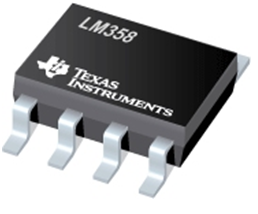
\includegraphics[width = .40\textwidth]{Figures/13.jpg}
 \caption{IR Sensor LM358}
 \label{ir}
\end{figure}

The LM358 specifies that it consists of two independent, high gain, internally frequency compensated operational amplifiers which were designed specifically to operate from a single power supply over a wide range of voltages. Operation from split power supplies is also possible and the low power supply current drain is independent of the magnitude of the power supply voltage. The LM358 is available in a chip sized package (8-Bump micro SMD) using National’s micro SMD package technology.
\subsubsection{Features}
\begin{enumerate}
 \item Available in 8-Bump micro SMD chip sized package, (See AN-1112)
\item Internally frequency compensated for unity gain
\item Large dc voltage gain: 100 dB
\item Wide bandwidth (unity gain): 1 MHz (temperature compensated)
\item Wide power supply range:
\item single supply: 3V to 32V
\item dual supplies: ±1.5V to ±16V
\item Very low supply current drain (500 $\mu$A)—essentially independent of supply voltage
\item Low input offset voltage: 2 mV
\item Input common-mode voltage range includes ground
\item Differential input voltage range equal to the power supply voltage
\item Large output voltage swing
\end{enumerate}

\subsubsection{Applications} 
\begin{enumerate}
 \item Active Filters 
 \item General Signal Conditioning and Amplification
 \item 4-mA to 20-mA Current Loop Transmitters
\end{enumerate}


\newpage
\vspace*{\fill}
 \begin{center}
\hrule%
\vspace{1pt}%
\hrule
\vspace{1pc}%
\LARGE\MakeUppercase{MANUFACTURING} 
\vspace{1pc}%
\hrule%
\vspace{1pt}%
\hrule
 \end{center}
 \vspace*{\fill}

\chapter{MANUFACTURING}
\section{PCB Layout}
Layout basically means placing or arranging things in a specific order on the PCB. Layout means placing of components in an order. 
\begin{figure}[!h]
 \centering
 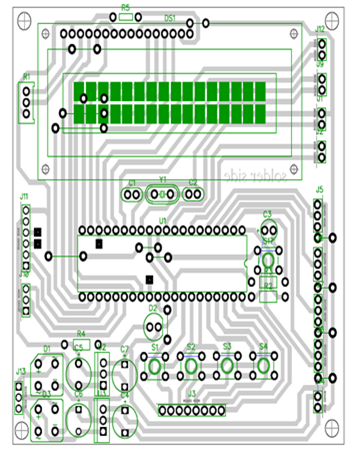
\includegraphics[width = .50\textwidth]{Figures/14.jpg}
 \caption{PCB Layout}
 \label{PCB Layout}
\end{figure}
This placement is made such that the interconnection lengths are optimal. At the same time, it also aims at providing accessibility to the components for insertion testing and repair.

The PCB layout is the starting point for the final artwork preparation layout design should reflect the concept of final equipment. There are several factors, which we must keep in mind for placing the layout. 

\subsection{Layout Methodology}
 For proper layout design minimal, steps to be followed are-
\begin{enumerate}
 \item Get the final circuit diagram and component list. 
\item Choose the board types, single sided / double sided / multilayered. 
\item Identify the appropriate scale for layout.
\item Select suitable grid pattern. 
\item Choose the correct board size keeping in view the constraints. 
\item Select appropriate layout technique, manual / automated. 
\item Document in the form of the layout scale.
\end{enumerate}

\subsection{PCB Construction}
The different processes that take place in the fabrication of a PCB are as follows:
\begin{enumerate}
 \item Layout designing
\item Transfer of pattern on copper board.
\item Drying 
\item Etching
\item Tinning
\item Drilling
\item Soldering
\item Surface cleaning
\end{enumerate}

\subsubsection{Layout designing}
First of all layout design of the circuit switch is to be traced on the PCB, is prepared. The layout of a PCB has to incorporate all the information on the board one can go to the art work preparation. The detailed circuit diagram is very important for the layout designer but he must also familiar with the design concept \& with the philosophy behind the equipment. In this process the layout designer, traces the circuit on a graph paper. By this process he marks where the holes should be. Thus the circuit, which is to be traced on the PB, is firstly traced on the graph paper or its layout is designed. In layout designing the distance between the copper tracks \& length, size etc. of components are also taken into consideration.
\subsubsection{Transfer of pattern on copper board}
After designing the art work on the graph paper, we transferred it onto the trace paper. The conductor pattern is then transferred n to the copper clad lamination with the help of carbon paper. By this the pattern gets transferred on the copper clad lamination.
\subsubsection{Etching}
Etching is done to remove all the unwanted copper which is present on the portion other than the pattern on the PCB. For this the PCB is kept dipped in the solution (FeCl2) \& two or three drops of HCL. The chemicals react with copper \& dissolve it. After some hours of time we get the PCB left with only copper tracks on it.
\subsubsection{Tinning}
The board is tinned using a soldering iron and a small piece of tinned solder wick. Tinning isn't absolutely necessary but it improves the appearance of the board, and prevents the copper from oxidizing before it's time to solder the parts to the board.
\subsubsection{Drilling}
Drilling of component mounting holes into PCB is the most important mechanical matching operation in PCB production process. Holes are made by drilling where ever a superior hole finish in is required. Therefore, drilling is applied by all the professional grade PCB manufacturers \& generally in all smaller PCB production plants \& laboratories.
\subsubsection{Soldering}
Soldering is the process of joining two metallic conductors, the joint where the two metallic conductors are to be joined or fused is heated with a device called soldering iron and then an alloy of tin and lead called solder is applied which melts and cover the joint. The solder cools and solidifies quickly to ensure a good and durable connection between the joined metals. Covering the joint with solder prevents oxidation.
\subsubsection{Surface cleaning}

\subsection{Equipments Required}
The various tools and equipments required for construction of a PCB are given below
\begin{enumerate}
 \item Solder kit consist of :
 \begin{enumerate}
  \item Soldering iron. 
  \item Soldering wire. 
  \item Flux
 \end{enumerate}
\item Tweezer
\item Cutter
\item Multi-meter (Measuring instrument).
\end{enumerate}

There are several factors, which we must keep in mind for placing the layout.
\begin{itemize}
 \item \textbf{Schematic diagrams:} The schematic diagrams forms main input document for preparation of the layout for this purpose the software for PCB design Express PCB was used. 
\item \textbf{Electrical and thermal requirement:} The PCB designer must aware of the circuit performance in critical aspects of the same concerning electrical conditions and the environment to be used. 
\item \textbf{Components and placing requirement:} All components are too placed in a configuration that demands only the minimum length for critical conductors. These key components are placed first and the other are grouped around like satellites.
\item \textbf{Mechanical requirement:} The designer should have the information about physical size of the board, type of installation of board (vertical/horizontal). The method of cooling adopted, front panel operated components etc.
\end{itemize}

\section{Software Used}
Microcontroller programming:
\begin{enumerate}
 \item Embedded  C
 \item MPLAB IDE compiler 
  \item PIC kit  
  \item Proteus 7 professional
\end{enumerate}

\subsection{MPLAB IDE Features}
MPLAB IDE is a Windows® OS based Integrated Development Environment for the PIC micro MCU families and the PIC Digital Signal Controllers. The MPLAB IDE provides the ability to:
\begin{enumerate}
\item Create Project
\item Building The Project
\item Assemble Source Code
\item Testing Code With The Simulator
\end{enumerate}

\subsubsection{Create Project}
MPLAB Project Wizard will be used to Create a Project.

A project is the way the files are organized to be compiled and assembled. We will use a single assembly file for this project and a linker script. Choose Project>Project Wizard. From the Welcome dialog, click on Next> to advance. The next dialog (Step One) allows you to select the device, which we’ve already done. Make sure that it says PIC16F877A. If it does not, select the PIC16F877A from the drop down menu. Click Next>.

\begin{figure}[!h]
 \centering
 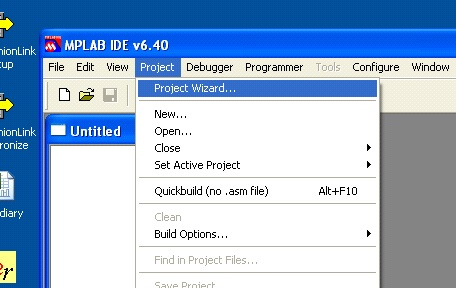
\includegraphics[width = .80\textwidth]{Figures/15.jpg}
 \caption{Starting Window}
 \label{Starting Window}
\end{figure}

MPLAB IDE is a Windows® OS based Integrated Development Environment for the PIC micro MCU families and the PIC Digital Signal Controllers
\newpage
\subsubsection{Select Tool}
Following fig. shows required tool to be selected:
\begin{figure}[!h]
 \centering
 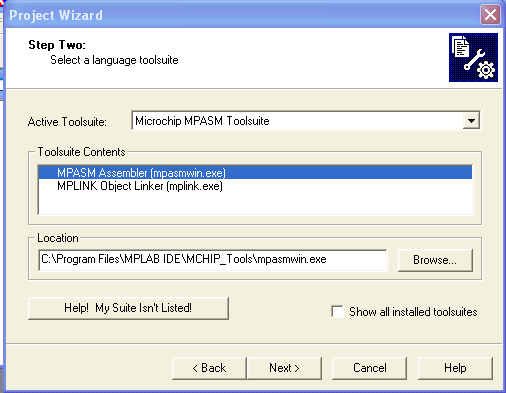
\includegraphics[width = \textwidth]{Figures/16.jpg}
 \caption{Select Tool}
 \label{Select Tool}
\end{figure}

\subsubsection{Adding Files To The Project}
Step Four of the Project Wizard allows file selection for the project. A source file has not yet been selected, so we will use an MPLAB IDE template file. The template files are simple files that can be used to start a project. They have the essential sections for any source file, and contain information that will help you write and organize your code. These files are in the MPLAB IDE folder, which by default is in the Program Files folder on the PC. There is one template file for each Microchip PICmicro and dsPIC device. Choose the file named f452tmpo.asm. If MPLAB IDE is installed in the default location, the full path to the file will be:

\begin{enumerate}
 \item \textbf{Naming the Project}
\begin{figure}[!h]
 \centering
 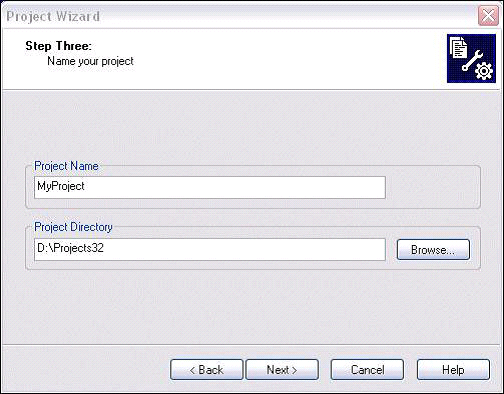
\includegraphics[width = \textwidth]{Figures/17.jpg}
 \caption{Naming the Project}
 \label{Naming the Project}
\end{figure}
\item \textbf{Building the Project}\\
From the Project menu, we can assemble and link the current files. They don’t have any of our code in them yet, but this assures that the project is set up correctly.
To build the project, select either:
\begin{enumerate}
 \item Project>Build All
\item Right-click on the project name in the project window and select Build All
\item Click the Build All icon on the Project toolbar. Hover the mouse over icons to see pop-up text of what they represent.
\end{enumerate}
\newpage
\item \textbf{Creating Code}
\begin{figure}[!h]
 \centering
 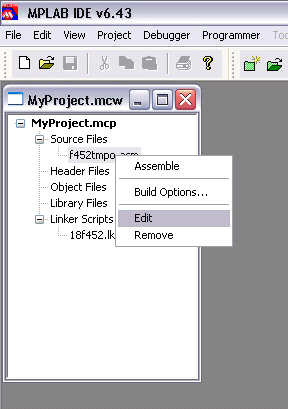
\includegraphics[width = .40\textwidth]{Figures/18.jpg}
 \caption{Creating Code}
 \label{Creating Code}
\end{figure}

\item \textbf{Assemble Source Code}\\
Following fig shows assemble source code as below:
\begin{figure}[!h]
 \centering
 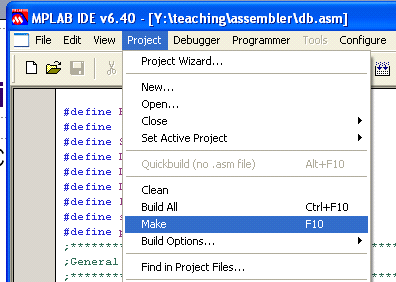
\includegraphics[width = .80\textwidth]{Figures/19.jpg}
 \caption{Assemble Source Code}
 \label{Assemble Source Code}
\end{figure}

\end{enumerate}
\subsubsection{Testing Code with the Simulator}
In order to test the code, software or hardware is needed that will execute the PIC micro instructions. A debug execution tool is a hardware or software tool that is used to inspect code as it executes a program (in this case cnt452.asm). Hardware tools such as MPLAB ICE or MPLAB ICD 2 can execute code in real devices. If hardware is not available, the MPLAB simulator can be used to test the code. For this tutorial use MPLAB SIM simulator. The simulator is a software program that runs on the PC to simulate the instructions of the PIC micro MCU. It does not run in “real time,” since the simulator program is dependent upon the speed of the PC, the complexity of the code, overhead from the operating system and how many other tasks are running. However, the simulator accurately measures the time it would take to execute the code if it were operating in real time in an application. Select the simulator as the debug execution tool. This is done from the Debugger>Select Tool pull down menu. After selecting MPLAB SIM, the following changes. 
\begin{itemize}
 \item The status bar on the bottom of the MPLAB IDE window should change to “MPLAB SIM”. 
\item Additional menu items should now appear in the Debugger menu. 
\item Additional toolbar icons should appear in the Debug Tool Bar.
\end{itemize}

\textbf{Simulator:}\\
 If you go to the debug menu, and select the simulator tool then you can simulate the running of your program using an emulator.

\section{Circuit Implementation}
\begin{enumerate}
 \item \textbf{Schematic Diagram:} The schematic diagram forms main input document for preparation of the layout. For this purpose the software for PCB design, Diptrace was used.
\item \textbf{Electrical and thermal requirement:} The PCB designer must be aware of the circuit performance in critical aspects of the same concerning electrical conditions and the environment to be used in.
\item \textbf{Mechanical requirement:} The designer should have the information about physical size of the board, type of installation of board (vertical/horizontal). The method of cooling adopted, front panel operated components etc. 
\item \textbf{Component placing requirement:} All component are to placed first in a configuration that demands only the minimum length for critical conductors. These key components are placed first and the others are grouped around like satellites. 
\end{enumerate}
\begin{figure}[!h]
 \centering
 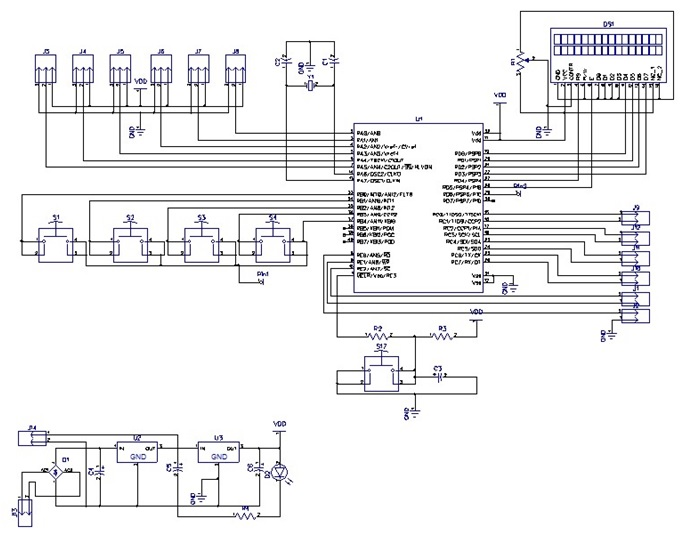
\includegraphics[width = \textwidth]{Figures/20.jpg}
 \caption{Circuit Implementation}
 \label{Circuit Implementation}
\end{figure}

\subsection{Art Work}
Art work is accurately scaled configuration of the printed circuit from which the master pattern is made photographically. 
\subsubsection{Art Work Rules}
Rules followed while selecting artwork symbol takes 
\begin{enumerate}
 \item Minimum spacing between conductor and pad should be 0 / 35 mm in 1:1 scale. 
\item Minimum spacing between parallel conductors should be 0.4 mm in 1:1 scale. 
\item The area of non-PTH solder pad should not be less than 5 sq.mm. 
\item The width of current carrying conductors should be determined for max.temp. rise of 20 ْ C.
\end{enumerate}
\subsubsection{General Art Work Rules}
\begin{enumerate}
 \item When there is higher conductor density assumes the conductors parallel to any one of the edge of the board 
\item When conductors have to be placed in other direction preference should be given to the 45ْ direction or to the 30ْ / 60ْ direction. 
\item Whenever there is sufficient space available the conductors can be run in any direction so as to achieve sorted possible interconnection. 
\item As far as possible, design and the conductor on the solder pad. 
\item Conductor forming sharp internal angles must be avoided. 
\item When a member of conductor has to run between two pads the conductor lines are run perpendicular w.r.t. the center-to-center line of pair of pads. 
\item Equally distributed spacing is to be provided when three or more conductors run along a direction and / or between two pads. 
\item Minimum spacing is provided when three or more lines run along a direction and / or between two pads.
\item The diameter of solder pad should be approximately 8 times the drilled hole diameter.
\end{enumerate}

\subsection{Crystal Circuit}
Pins OSC1 \& OSC2 are provided for connecting a resonant network to form oscillator. Typically a quartz crystal and capacitors are employed. The crystal frequency is the basic internal clock frequency of the microcontroller.
\begin{figure}[!h]
 \centering
 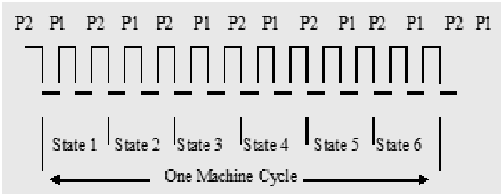
\includegraphics[width = .60\textwidth]{Figures/21.jpg}
 \caption{Crystal Cycles}
 \label{Crystal Cycles}
\end{figure}
The manufacturers make available designs that can run at specified maximum \& minimum frequencies, typically 1MHz to 32MHz. Here we are connecting two ceramic capacitors which are basically used for filtering. In other words to give a pure square wave to the $\mu$C we are connecting the two capacitors. The basic rule for placing the crystal on the board is that it should be as close to the $\mu$C as possible to avoid any interference in the clock.

\subsection{MAX-232}
Many device today work on RS 232 logic such as PC, GSM modem, GPS etc.  So in order to communicate with such devices we have to bring the logic levels to the 232 logic (+/-9V). Here as we can see the RS 232 chip has 2 pairs of TTL and 232 logic; which are:
\begin{enumerate}
 \item Pair 1 : Pin 7,8,9,10 of RS 232
\item Pair 2 : Pin 11,12,13,14  of RS 232
\end{enumerate}
\begin{figure}[!h]
 \centering
 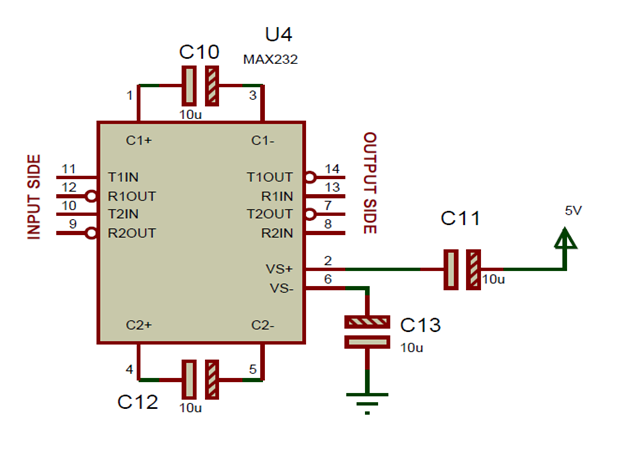
\includegraphics[width = \textwidth]{Figures/22.jpg}
 \caption{Interfacing  of MAX232}
 \label{Interfacing  of MAX232}
\end{figure}
We can use any one pair in our project either 7, 8,9,10 pair or 11,12,13,14 pair. if we require 2 serial ports then Depending on the requirement of the project we may have to use both the pair in the same project. The $\mu$C works on TTL logic (0-5V). So to convert the TTL logic to 232 logic we use the 4 capacitors connected to the RS232 IC. These capacitors are called charge pumps used to convert the TTL voltage to the +/- 9V swing required by the 232 IC.

\subsubsection{Dual Charge-Pump Voltage Converter}
The MAX220–MAX249 have two internal charge-pumps that convert +5V to ±10V (unloaded) for RS-232 driver operation. The first converter uses capacitor C1 to double the +5V input to +10V on C3 at the V+ output. The second converter uses capacitor C2 to invert +10V to -10V on C4 at the V- output.

\subsection{LCD Section}
16x2 Character LCD is a very basic LCD module which is commonly used in electronics projects and products. It contains 2 rows that can display 16 characters. Each character is displayed using 5×8 or 5×10 dot matrix. It can be easily interfaced with a microcontroller. In this tutorial we will see how to write data to an LCD with PIC Microcontroller using Hi-Tech C Compiler. Hi-Tech C has no built in LCD libraries so we require the hardware knowledge of LCD to control it. Commonly used LCD Displays uses HD44780 compliant controllers.

Below shown , is the pin diagram of a 16x2 Character LCD display. 
\begin{figure}[!h]
 \centering
 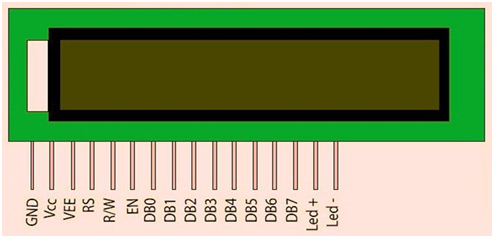
\includegraphics[width = .70\textwidth]{Figures/7.jpg}
 \caption{2 * 16 LCD}
 \label{lcd}
\end{figure}
As in all devices it also has two inputs to give power Vcc and GND. Voltage at VEE determines the Contrast of the display. A 10K potentiometer whose fixed ends are connected to Vcc, GND and variable end is connected to VEE can be used to adjust contrast. A microcontroller needs to send two information to operate this LCD module, Data and Commands. Data represents the ASCII value (8 bits) of the character to be displayed and Command determines the other operations of LCD such as position to be displayed. Data and Commands are send through the same data lines, which are multiplexed using the RS (Register Select) input of LCD. When it is HIGH, LCD takes it as data to be displayed and when it is LOW, LCD takes it as a command. Data Strobe is given using E (Enable) input of the LCD. When the E (Enable) is HIGH, LCD takes it as valid data or command. The input signal R/W (Read or Write) determines whether data is written to or read from the LCD. In normal cases we need only writing hence it is tied to GROUND in circuits shown below.

\subsection{Power Supply}
\subsubsection{5V Supply Design}
The +5 volt supply is useful for both analog and digital circuits. DTL, TTL, and CMOS ICs will all operate nicely from a +5 volt supply. In addition, the +5 volt supply is useful for circuits that use both analog and digital signals in various ways.
\begin{figure}[!h]
 \centering
 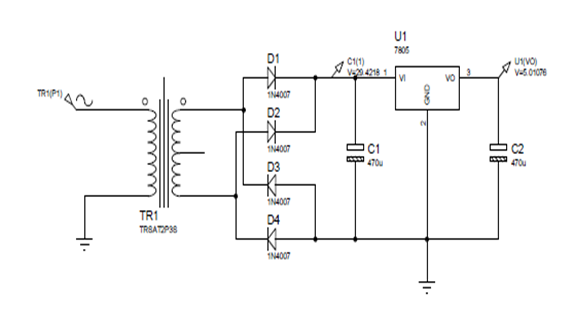
\includegraphics[width = \textwidth]{Figures/24.jpg}
 \caption{Design of Power Supply}
 \label{Design of Power Supply}
\end{figure}

The +5 volt supply is based on the commercial 7805 voltage regulator IC . This IC contains all the circuitry needed to accept any input voltage from 8 to 18 volts and produce a steady +5 volt output, accurate to within 5\% (0.25 volt). 
It also contains current limiting circuitry and thermal overload protection , so that the IC won’t be damaged in case of excessive load current; 
it will reduce its output voltage instead. The 10 $\mu$f and 0.01 $\mu$f capacitors serve to help keep the power supply output voltage constant when load conditions change. The electrolytic capacitor smooth ot any longterm or low frequency variations. However, at high frequencies this capacitor is not very efficient, therefore, the 0.01$\mu$f is included to bypass high frequency changes, such as digital IC switching effects, to ground. We can select a 15V secondary Voltage. In our system most of the components used require 5V as operating voltage such as micro controller, MAX 232, MCT2E etc. The total current, which our circuit sinks from the power supply, is not more than 100 mA. We have used Regulator IC 7805 that gives output voltage of 5V. The minimum input voltage required for the 7805 is near about 7V. Therefore we have used the transformer with the voltage rating 230V-10V and current rating 500mA. The output of the transformer is 12V AC. This Ac voltage is converted into 12V DC by Bridge rectifier circuit. 
The reasons for choosing the bridge rectifier are :
\begin{itemize}
 \item The TUF is increased to 0.812 as compared the full wave rectifier.
\item The PIV across each diode is the peak voltage across the load =Vm, not 2Vm as in the two diode rectifier
\end{itemize}

Output of the bridge rectifier is not pure DC and contains some AC some AC ripples in it. To remove these ripples we have used capacitive filter, which smoothens the rippled out put that we apply to 7805 regulators IC that gives 5V DC. We preferred to choose capacitor filters since it is cost effective, readily available and not too bulky.

\subsubsection{Advantages}
\begin{enumerate}
 \item Mistakes in tool settings are practically eliminated and tool configuration time is minimized.
\item This allows you to quickly access all your development tools (development tools and third-party tools) from a single environment. All configuration details are saved in the µVision project.
\item Accelerates application development. While editing, you may configure debugger features. While debugging, you may make source code modifications.
\item Accelerates application development. While editing, you may configure debugger features. While debugging, you may make source code modifications.
\end{enumerate}








\newpage
\vspace*{\fill}
 \begin{center}
\hrule%
\vspace{1pt}%
\hrule
\vspace{1pc}%
\LARGE\MakeUppercase{EXPERIMENTATION} 
\vspace{1pc}%
\hrule%
\vspace{1pt}%
\hrule
 \end{center}
 \vspace*{\fill}

\chapter{EXPERIMENTATION}

\section{Flowchart of system}
The working starts with the initialization of the system. When the patient is brought in the ambulance, 
\begin{figure}[!h]
 \centering
 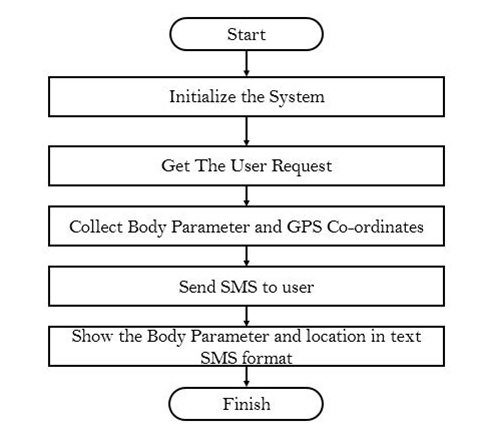
\includegraphics[width = .70\textwidth]{Figures/25.jpg}
 \caption{Flowchart of system}
 \label{Flowchart of system}
\end{figure}
all the medicinal equipments and the sensors (like heartbeat and temperature) are being used to collect the status and physical condition of the patient with the help of readings given by these sensors along with the gps co-ordinates of the ambulance.

All these informations are sent to the hospital using the gsm module which will show all the body parameters and the location of the ambulance on the screen connected to the receiver. 

\section{Program}
\lstinputlisting[language=C]{Main.c}


\newpage
\vspace*{\fill}
 \begin{center}
\hrule%
\vspace{1pt}%
\hrule
\vspace{1pc}%
\LARGE\MakeUppercase{RESULTS} 
\vspace{1pc}%
\hrule%
\vspace{1pt}%
\hrule
 \end{center}
 \vspace*{\fill}

\chapter{RESULTS}
\section{Traffic Light Simulation}
\begin{figure}[!h]
 \centering
 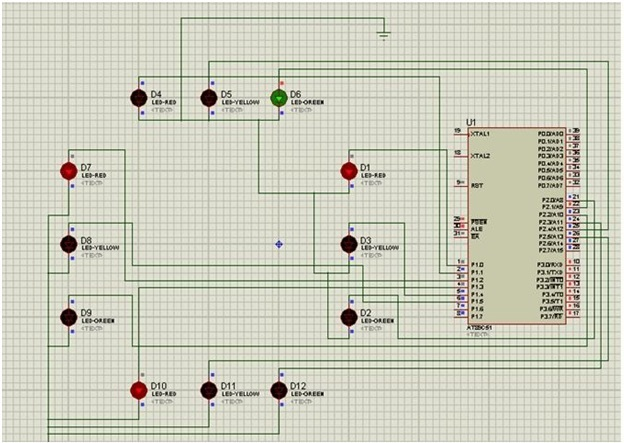
\includegraphics[width = \textwidth]{Figures/26.jpg}
 \caption{Software Simulation}
 \label{Software Simulation}
\end{figure}
The traffic signals are being controlled by the microcontroller using RF transmitter, connected to the ambulance unit, and RF receiver, present at the traffic signals. The RF transmitter connected to the ambulance is continuously transmitting signal. When it comes in range with the receiver, the receiver detects the signal and changes the traffic signal to green.

\section{Simulations}
The output of LCD can be seen in figure. The LCD shows the readings of patient’s temperature and heart rate/ heart beat.
\begin{figure}[!h]
 \centering
 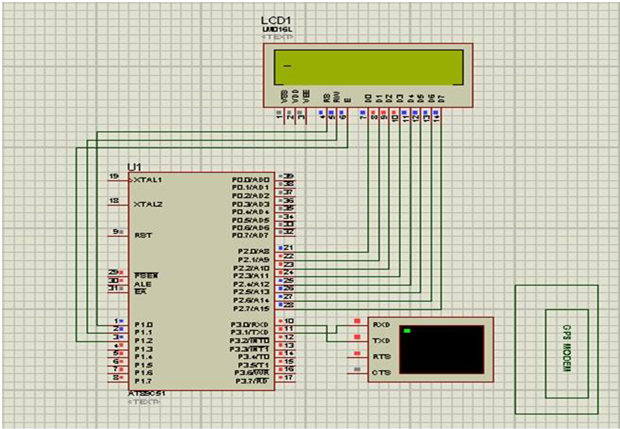
\includegraphics[width =\textwidth,height=12cm]{Figures/27.jpg}
 \caption{Simulation for LCD}
 \label{Simulation for LCD}
\end{figure}

All the parameters that is being recorded of the patient in the ambulance is being displayed at the LCD present in the ambulance. The LCD receives data to be displayed, from the microcontroller that itself obtains receives those data from the sensors.

The gsm is used so as to establish communication between the ambulance and the hospital unit. All the data recorded along with the location of the ambulance can be provided to the hospital so as to make the arrangements possible prior to the time  the patient reaches the hospital.
\begin{figure}[!h]
 \centering
 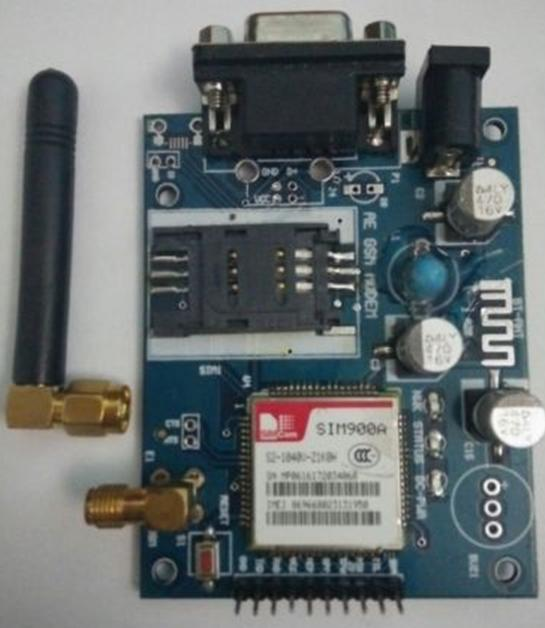
\includegraphics[height = .70\textwidth, angle=90]{Figures/28.jpg}
 \caption{Snapshot of system}
 \label{Snapshot of system}
\end{figure}

  
\begin{figure}[!h]
 \centering
 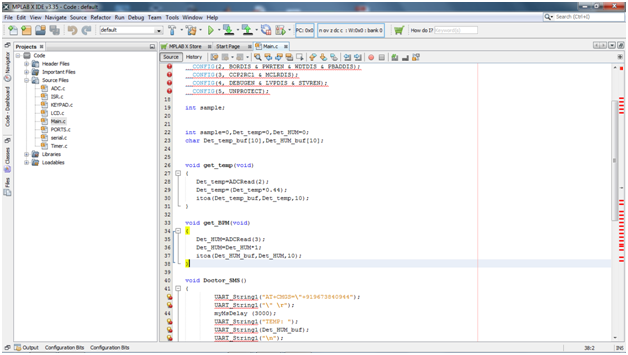
\includegraphics[width = \textwidth]{Figures/30.jpg}
 \caption{workspace 1}
 \label{workspace 1}
\end{figure}

Using the codes shown above in the fig., different parameters of patient’s body functioning are being recorded in the memory unit, using different sensors such as heartbeat sensor, or, the temperature sensor. These data are then sent from the microcontroller to the hospital unit using gsm module. 

\begin{figure}[!h]
 \centering
 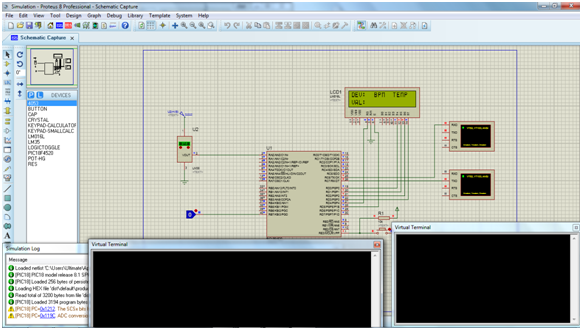
\includegraphics[width = \textwidth]{Figures/31.jpg}
 \caption{Simulation result 1}
 \label{Simulation result 1}
\end{figure}

\begin{figure}[!h]
 \centering
 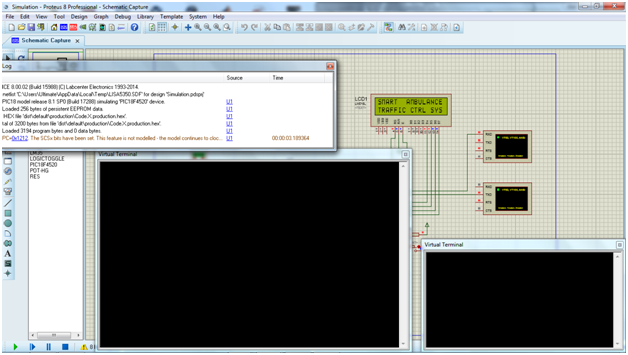
\includegraphics[width = \textwidth]{Figures/32.jpg}
 \caption{Simulation result 2}
 \label{Simulation result 2}
\end{figure}

The above diagram in Figure:\ref{Simulation result 1}, shows the result of the complete processing of the system. The microcontroller acts as the controlling body of the system. It controls the devices and also keeps a check on the connections formed for the transmission and reception of data.

Figure:\ref{Simulation result 2} the runtime simulation result. As can be seen in the diagram, the lcd is connected to the microcontroller, which will send the data to the LCD , displaying the name of the project. 

\section{Benefits}
\begin{enumerate}
 \item Information of the patient is available right from the place where the patient is picked up by the ambulance.
\item Traffic signals can be controlled well before 100m of the chowk.
\item Very basic and essential parameters like, Blood pressure, heart rate, body temperature are analysed and transmitted.
\item GSM unit is very much reliable and data transmission is faster.
\item Convenience in readability for parameters at the hospital unit , as using VB.
\item NO separate coding required for different chowks and lanes.
\end{enumerate}

\section{Applications}
\begin{enumerate}
 \item The concept of wireless transmission of data can be used not only in medical field but also in industrial field for transmission of information regarding a particular m/c.
\item In very immense and critical situations where in humans can’t be physically present. Ex.    Coal mines, Nuclear power plants.
\item Defence field, for sending the parameters of the soldier to the base station. 
\item Can be used for VIP cars. 
\item Traffic management and control.
\item Fire Extinguishing vehicle. 
\item Police van in emergency cases
\end{enumerate}

\section{Advancements}
\begin{enumerate}
 \item Real time continuous wireless patient monitoring system. 
\item 3G Technology,3.5G Technology,4G technology. 
\item Centralized signalling station for traffic control.
\end{enumerate}

\newpage
\vspace*{\fill}
 \begin{center}
\hrule%
\vspace{1pt}%
\hrule
\vspace{1pc}%
\LARGE\MakeUppercase{CONCLUSION} 
\vspace{1pc}%
\hrule%
\vspace{1pt}%
\hrule
 \end{center}
 \vspace*{\fill}

\chapter{CONCLUSION}
After getting the specified parameter by using sensors then it will get notified to the doctors by receiving message through GSM.IR sensors are used to manage and control traffic. The system is to provide important medical facilities and help the hospital prepare well before the patient reaching the hospital via MAX 232. Along with this, using IR sensors to control the traffic on the way up to the hospital. The MPLAB software is interfaced to the ambulance unit as well as to the hospital unit. The microcontroller , which acts as a controlling unit, is interfaced with Sensors (heartbeat, temperature, IR ) to record the condition of the patients send these information to the hospital, and also help the ambulance get through the traffic signals without any hindrances.
\section{Future Scope}
This project of infrared traffic light system is one of the best ways to smoothen the journey of an emergency vehicle. However, this system can be improved in future by designers. Some of the ideas are mentioned below :
\begin{enumerate}
 \item The using of laser diode instead of using the light emitting diode (LED) because the laser   diode has wide modulation bandwidths. The infrared can be transmitted in longer range by using the laser diode rather than the LED. 
\item The using of radio frequency (RF) to change the using of infrared transmission. With radio frequency, the radio wave is transmitted in radius and it is more practical.
\end{enumerate}


%---------------------------------------------------------------------------------------------------------------------
% References
%---------------------------------------------------------------------------------------------------------------------
\addcontentsline{toc}{chapter}{Bibliography}
\begin{thebibliography}{29}
\bibitem{1}
Ankit Jha, Lalit Kanwar, Mayur Solanki, Shyam Sunder Joshi , Smt. Sarita Chauhan, “An  Advance Intelligent Ambulance With Online Patient Monitoring System”, \textit{IPASJ    International Journal of Electronics \& Communication (IIJEC)}, Vol. 3, Issue 4, April 2015.

\bibitem{2}
Dr. Shantanu  K. Dixit, Miss. Ashwini A. Joshi, “A  Review Paper on Design of GPS and GSM  Based  Intelligent Ambulance”, \textit{Monitoring  International  Journal  of  Engineering Research  and  Applications},  Vol. 4, Issue 7( Version 6), July  2014.

\bibitem{3}
Mohd Azwan Azim Rosli, Mohd Helmy Abd Wahab*, Rahmat Sanudin, Mohd Zainizan, “A Hardware basd approach in designing Infrared Traffic Light System”.
\bibitem{4}
GargiBeri, PankajGanjare, Amruta Gate, AshwinChannawar’s, “Intelligent Ambulance with Traffic Control”.
\bibitem{5}
Miss. Ashwini , A. Joshi Int, “A Review Paper on Design of GPS and GSM Based Intelligent Ambulance Monitoring”, \textit{Journal of Engineering Research and Applications}.
\bibitem{6}
Manoj Prabhakar S and Manoj Kumar, “GPS Tracking System Coupled With IMAGE PROCESSING IN TRAFFIC SIGNALS“.
\bibitem{7}
Ms Sarika B. Kale Gajanan P. Dhok’s, “EMBEDDED SYSTEM For Intelligent Ambullance and Traffic Control Management” \textit{IJCER}, Vol 2, Issue 2, 2013.
\bibitem{8}
Megha A. Tank, Hardik Mewada, Viraj Chokes, “ Review on Smart Traffic control for Emergency Vehicles” \textit{IJCA}, vol 117, Issue 7 , 2015.
\bibitem{9}
Veera V. Venkatesh , Nazeen Syed, “Smart Traffic Control System for Emergency  Vehicle”,\textit{IJIR}, Vol 3,Issue 8 , Aug 2015.
\bibitem{10}
S Sharma, A Pithvora, G Gupta, M Goel and M Sinha’s, “Traffic Light Priority Control For Emergency Vehicle Using RFID”.
\end{thebibliography}
\end{document}


